\section{Online}
\label{sec:online}

In the online part of the approach, the artifacts present in the repository are autonomously deployed to the target computing environment.

\begin{figure*}[!htb]
  \centering
  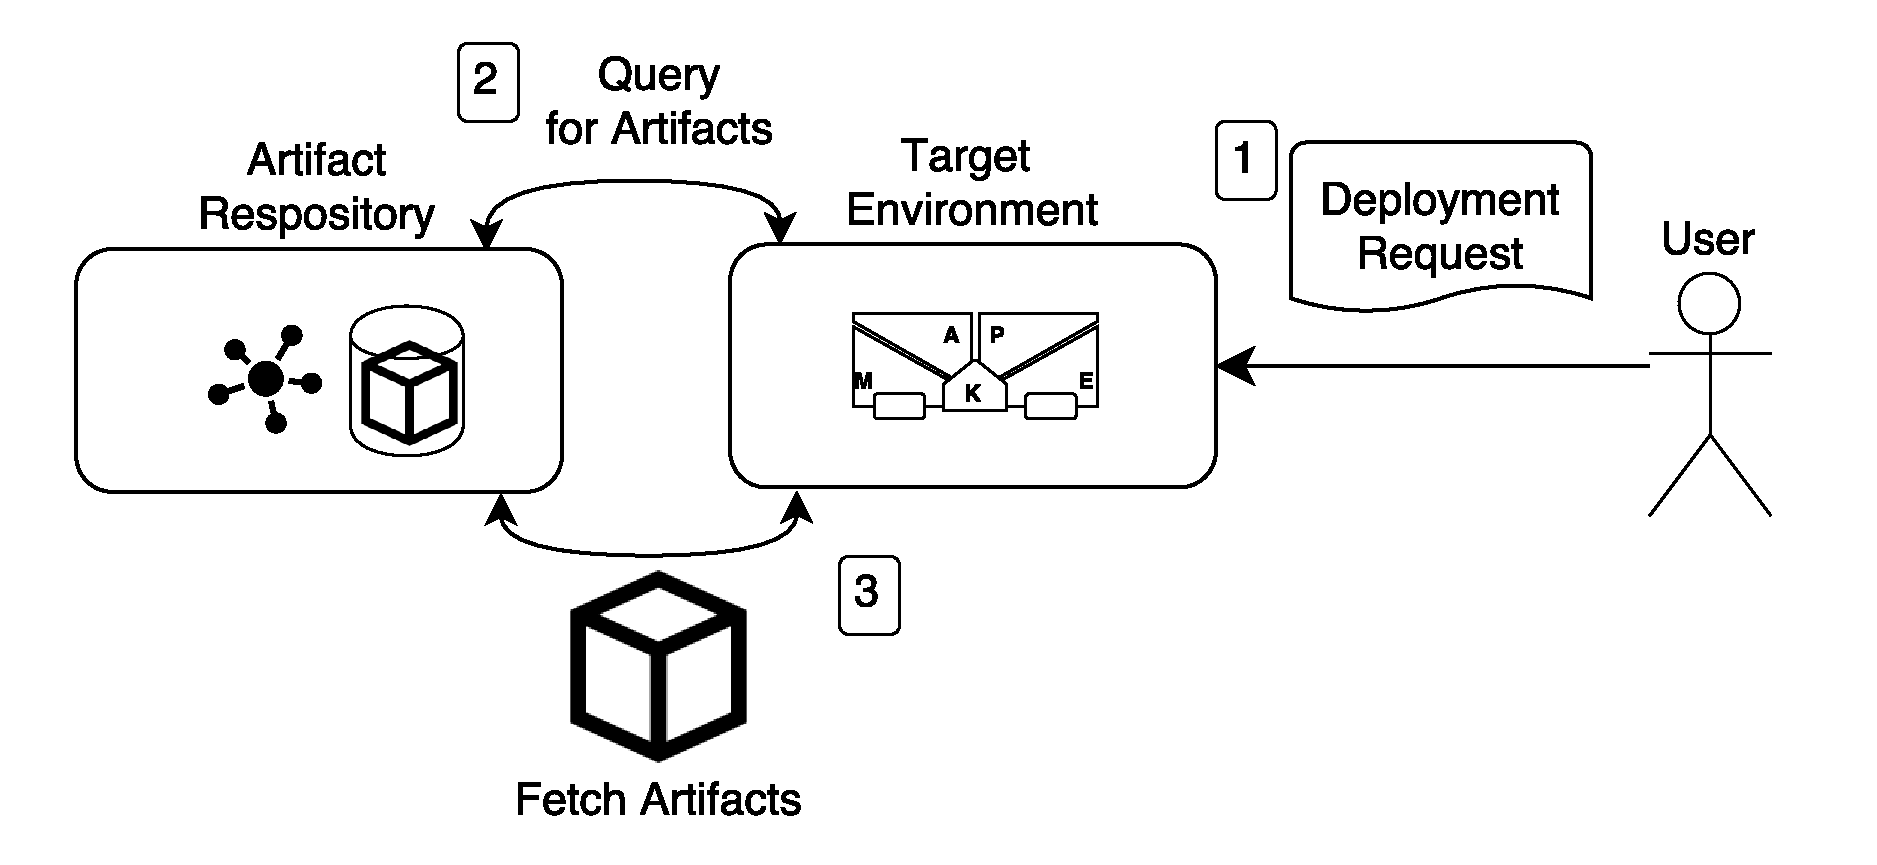
\includegraphics[width=1\linewidth]{deployment_actors}
  \caption{Goald Autonomic Deployment}
\label{fig:deployment_actors}
\end{figure*}

Figure~\ref{fig:deployment_actors} depicts the online activities. A user interested in using a computing environment to achieve a set of goals submits to such environment which goals it wants to achieve in the form of a deployment request. Then, the system analyzes the available computing resources and artifacts present in the repository then plan the deployment, generating a deployment plan that is a selection of artifacts that can allow for the goals achievement in the available computing environment. The deployment is then executed by fetching the appropriate artifacts from the repositories.

\subsection{Autonomic Deployment Planning}
\label{sec:planning}

The deployment planning is the core of the online part of the presented approach. Its objective is to solve the variability present in the design, allowing the system to adapt to the target computing environment. It is executed autonomously in the target environment. In this Section~\ref{sec:metamodel} is presented the metamodel used and in Section~\ref{sec:algorithm} an algorithm to come up with a deployment plan.

\subsubsection{Metamodel}
\label{sec:metamodel}

\begin{figure}[!htb]
  \centering
  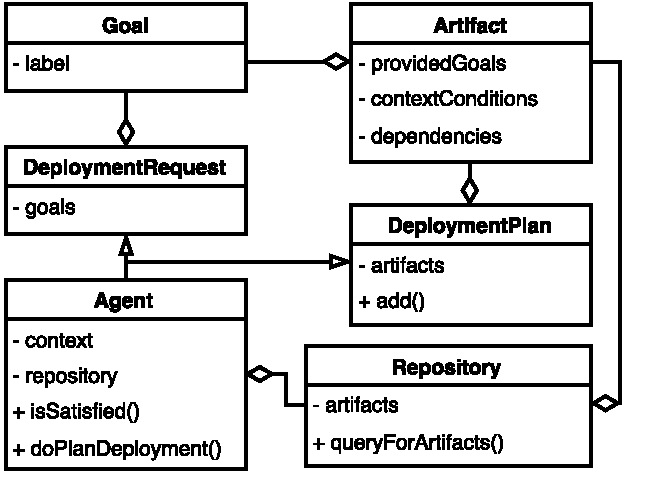
\includegraphics[width=0.7\linewidth]{metamodel}
  \caption{The Goalp Deployment metamodel}
  \label{fig:metamodel}
\end{figure}

Figure~\ref{fig:metamodel} presents the metamodel used. \emph{Artifact} is the central entity at deployment level. As described in the Section~\ref{sec_artifacts}, artifacts have \emph{provided goals}, \emph{context conditions}, and \emph{dependencies} which create relations of dependency between artifacts, so that an artifact that has a goal dependency is dependent on an artifact that provides such goal. % However, this dependency is loose. An artifact do not depend on one specific other artifact, but instead, on any artifact that provides a goal.

An \emph{agent} can accept deployment requests, an action that should trigger the deployment planning. An agent knows a \emph{repository} where it looks for artifacts.
A \emph{repository} has a set of artifacts that it can be queried about by the \texttt{queryForArtifacts} method. The method \texttt{queryForArtifacts} receives a goal as the argument and return all artifacts in the repository that provide that goal. An \emph{agent} can verify \emph{context conditions} by \emph{isSatisfied} method.

The \emph{Deployment Request} is a set of goals that an external entity sends to an agent, requesting it to plan a deployment. \emph{Agent}’s \texttt{doPlanDeployment} method returns a \emph{Deployment Plan}, which is a set of  artifacts that provides the goals specified in the \emph{Deployment Request}.

Note that components do not appear here in this model. Components are architectural units that are packaged into artifacts. The components definitions are mapped and developed by the architect/developer offline, while components instantiation and binding are carried out in the online section.

Artifacts are \emph{deployable} for an agent if all its context conditions and dependencies are satisfiable.
Goals are \emph{achievable} if their artifacts are deployable as part of a deployment plan to achieve/fulfill such goals.

% \begin{figure}[!htb]
%   \centering
%   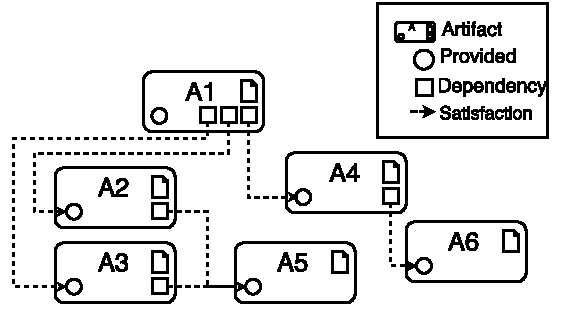
\includegraphics[width=.6\linewidth]{dependency_graph}
%   \caption{Dependency Graph}
% \label{fig:dependency_graph}
% \end{figure}

\subsubsection{Planning Method}
\label{sec:algorithm}

To come up with a deployment plan for a given deployment request and context, we present the Algorithm~\ref{plan_method}. It implements the \emph{Agent}'s \texttt{doPlanDeployment} method of Goalp metamodel.

\begin{algorithm}[!htb]
 \KwIn{DeploymentRequest request}
 \KwResult{DeploymentPlan plan}
  var resultingPlan $\leftarrow$ new DeploymentPlan() \;

  \ForEach{Goal selectedGoal in goals}{
    var subPlan $\leftarrow$ new DeploymentPlan() \;

    var artifacts $\leftarrow$ repository.
    \\queryForArtifacts(selectedGoal) \;

    \ForEach{Artifact artifact in artifacts}{
     	var contextSatisfaction $\leftarrow$ \\
      isSatisfied(artifact.contextConditions)\;

      \If{contextSatisfaction}{
        var plan $\leftarrow$ new DeploymentPlan ()\;

        plan.add(artifact)\;

        \If{artifact.dependencies == EMPTY}{
          subPlan.add(plan)\;

          break\;
        }\Else{
          var depPlan  $\leftarrow$ doPlanDeployment (artifact.dependencies)\;

          \If{depPlan != NULL}{
          plan.add(depPlan)\;

          subPlan.add(plan)\;

          break\;
          }
        }
      }
    }
    \If{subPlan != EMPTY}{
      resultingPlan.add(subPlan)\;

    }\Else{

      \Return{NULL}
    }
  }
  \Return{resultingPlan}

  \caption{doPlanDeployment (List goals)}
  \label{plan_method}
\end{algorithm}

The Algorithm~\ref{plan_method} works as follows: it receives as a parameter a deployment request, which contains a list of goals. For each goal in the list, it queries the repository for artifacts that provide this goal (line 4). The repository returns a list of artifacts. For each artifact, the algorithm looks for a sub-plan with this artifact (lines 5-21). First, the context conditions are verified (line 6). If the context is satisfied (line 7),
then a new plan is created with the artifact (lines 8-9). If the list of dependencies of the artifact in empty (line 10), them the new plan is added to the sub-plan (line 11). Else, if the artifact has a not empty set of dependencies, the algorithm is recursively called for these dependencies. If the results of the recursive call is not \texttt{NULL} (line 15), the resulting plan is added to the new plan and included into the sub-plan (lines 16-17).
In both cases that new plan is added to a sub-plan, the look for a deployment plan that satisfies the selected goal is over and the inner \texttt{for} loop is halted (lines 12 and 19) and then the sub-plan is added to the resulting plan (line 25).
Otherwise, if the context conditions evaluation (line 6) returns \texttt{FALSE} or the recursive call returns \texttt{NULL}, the artifact can not be deployed. The loops continue and other artifacts will be tried. If after all tries the sub-plan is \texttt{EMPTY} (line 27), the deployment for the selected goal is not possible, and the algorithm returns \texttt{NULL} (line 28). Note that the algorithm will return \texttt{NULL} if for any of the goals in the request it is not possible to come up with a plan. Otherwise, the algorithm will return a valid plan.

It could be the case that there is more than one possible valid plan. But this algorithm will return the first one found.  We let for future works the investigation of approaches to come up with the best alternative plan in case more than one is valid.

\subsubsection{Verifying a Plan}
\label{verify_plan}

A deployment plan, is \emph{valid} for a given context if: (i) for each artifact in the plan, for the current context, all context conditions hold.
(ii) for each artifact, for all its dependencies, there is at least one artifact in the plan that provides it (the dependency).

A deployment plan satisfies a deployment request if it is \emph{valid}, and (iii) for each goal, in the deployment request, there is at least one artifact that provides this goal.

Being so, we can verify if a deployment plan satisfies a deployment request by executing the following steps that verify properties (i), (ii) and (iii):

\begin{itemize}
  \item Check if for all selected artifacts, all context conditions are met.
  \item Check if for all selected artifacts, the dependencies are within the deployment plan.
  \item Check if for all goals in the deployment request there is at least one artifact that declares each intended goal and one that provides such goal.
\end{itemize}

\subsection{Deployment Execution}

The last step of the approach is the deployment execution. The deployment execution involves (i) copying the artifacts present in the deployment plan from the repository to the target environment. And (ii) binding together the components present into these artifacts, creating the application architecture.

To bind components, the Dependency Injection\cite{fowler_inversion_2004} design pattern can be used.
